\chapter{\label{CH:Pipeline}TuMag's pipeline and data.}


The 2024 observational campaign of the third edition of the Sunrise observatory was an outstanding success. In contrast to previous flights, where technical challenges severely limited the number of useful observations, all subsystems performed exceptionally well during this third flight, allowing for nearly continuous instrument operation over more than six days. From TuMag’s perspective, the campaign yielded approximately 10 terabytes of data, consisting of over 40 scientific observation blocks and 250 calibration observations.

The substantial volume of data recorded by the three instruments, of which TuMag captured the least (in digital space) due to the instrument’s nature, required that it be physically recovered on-site, as it could not be broadcasted from the observatory to the operations center. Recovery activities began immediately after landing and lasted until early August, during which all surviving components, along with the data vaults, were transported to Yellowknife, Canada, the nearest city to the landing site. The data vaults arrived at MPS in early August, where a backup was created before the data associated with each instrument was sent to the respective IP institution. TuMag’s data arrived at  IAA in late August, marking the official start of the reduction process.

The reduction process began by labeling all images and identifying the more than 600 000 images captured by TuMag. Once the observations were correctly identified, the reduction process commenced and, at the time of writing, remains ongoing. Due to the relevance of the pipeline development and results for this thesis, this chapter will provide an overview of TuMag's data and the state of its pipleine, although the results remain preliminary.

The discussion will begin by introducing TuMag’s various observing modes, both scientific and calibration, followed by a brief review of the observation campaign, outlining the different observation programs and their scientific objectives. The chapter will conclude with an examination of the data reduction process, detailing the pipeline and presenting some initial results. It is important to note that, due to the late arrival of the data, this thesis had to be written in parallel with the reduction process. Therefore, the results presented here are preliminary, and the final product may differ as additional reduction steps are incorporated.

\section{TuMag's observing modes}

With the purpose of simplifying the operation activities, TuMag operates through a series of so-called observing modes. The observing modes are a list of pre-configured settings tailored for various observations, including both calibration and scientific purposes. Each mode is designed to fulfill the specific objectives of the corresponding observation and enables nearly automatic operation of the instrument during flight.

\begin{table}
    \centering
   \begin{tabular}{cccccccc}
    \hline
    \hline
    Observing mode & Spectral lines  & $N_\lambda$ & $N_P$ & $N_a$& $N_c$ & $t_{eff} (s)$ & (S/N) \\
    \hline
    0s & Mg I $b_2$ 5172.7 \r{A} & 12 & 1 & 2 & 1 & 6.3 & 500\\ 
    0p & Mg I $b_2$ 5172.7 \r{A} & 12 & 4 & 16 & 1 & 37.62 & 1000\\
    1  & Mg I $b_2$ 5172.7 \r{A} &  10 & 4 & 16 & 1 & 31.81 & 1000\\
    2  & Fe I 5250.2 \r{A}, Fe I 5250.6 \r{A} &  8 & 4 & 16 & 1 & 23.4 & 1000\\
    3  & Fe I 5250.2 \r{A}, Fe I 5250.6 \r{A} & 5 & 2 & 20 & 1 & 10.04 & 1000\\
    4  & Mg I $b_2$ 5172.7 \r{A} & 3 & 4 & 10 & 10 & 54.01 & 2500\\
    5  & Fe I 5250.2 \r{A}, Fe I 5250.6 \r{A} & 3 & 4 & 10 & 10 & 53.60 & 2500\\ 
    \hline
    \hline
    \end{tabular}
    \caption{Scientific observing modes. From left to righ, the columns are: observing mode identiicator, measured spectral lines, number of wavelengths, of modulations, of accumulations, of cycles, the total timeand the polarimetric SNR.}
    \label{table: scientific observing modes}
\end{table}

A summary of the properties for each observing mode is provided in Table \ref{table: scientific observing modes}. There are four distinct modes designed to observe the magnesium line. Mode 0s performs a fast, extended scan of the spectral line using 12 wavelength samples: [-40, -30, -20, -10, 0, 10, 20, 30, 40, 50, 60, 65]\footnote{Sampling positions are given relative to the line core.}, with one modulation and two accumulations to maximize scanning speed. Mode 0p is similar to mode 0s but employs a full-vector modulation scheme, requiring 16 accumulations to ensure the required SNR. Mode 1 provides a shortened scan of the magnesium line, with measurements taken at [-30, -20, -10, -5, 0, 5, 10, 20, 30, 65], also utilizing a vectorial modulation scheme. Finally, mode 4 is a "deep" magnetic mode, featuring a highly reduced scan with only three samples at [-10, 0, 10], but with increased accumulations and cycles to enhance polarimetric sensitivity. 

Three observing modes are configured for the iron lines. Mode 2 employs a vectorial modulation scheme applicable to both iron lines, with sampling at [-12, -8, -4, 0, 4, 8, 12, 22] pm. Mode 3 uses a longitudinal modulation scheme, measuring only Stokes I and V, with samples taken at [-8, -4, 4, 8, 22] pm. Lastly, mode 5 closely resembles mode 4, but is configured for the iron lines, with sampling at [-8, 0, 8] pm. The only difference between these two modes is the sampling scheme.

Although most of the parameters are set up by the observing mode and cannot be changed, there are some configurable parameters that allow to slightly modify the observing modes to fit the specific goal of a particular. These parameters are the following:

Solo estos? o había más? 
\begin{itemize}
    \Myitem $\lambda _ {\text{rep}}$ : A parameter that allows to repeat all the observations carried out at every spectral position before changing wavelength. This parameter is employed for flat-field observations (see the following section). By default is set to 1.
    \Myitem Etalon offset : A parameter that allows for the introduction of a global shift to the spectral sampling by offsetting the absolute voltages (and thus, wavelengths) of the scan. This parameter was used to center the spectral line in shorter observing modes affected by solar rotation or other effects that might shift the spectral position. The default value is set to 0 V.
    \Myitem $N_a$ : Even though the number of accumulations is fixed in nominal observing modes, this parameter was set as configurable in order to allow modifications for faster observations when needed. The  default value depends on the observing mode.  
\end{itemize}



\begin{figure}[t]
    \begin{minipage}[c]{0.67\textwidth}
      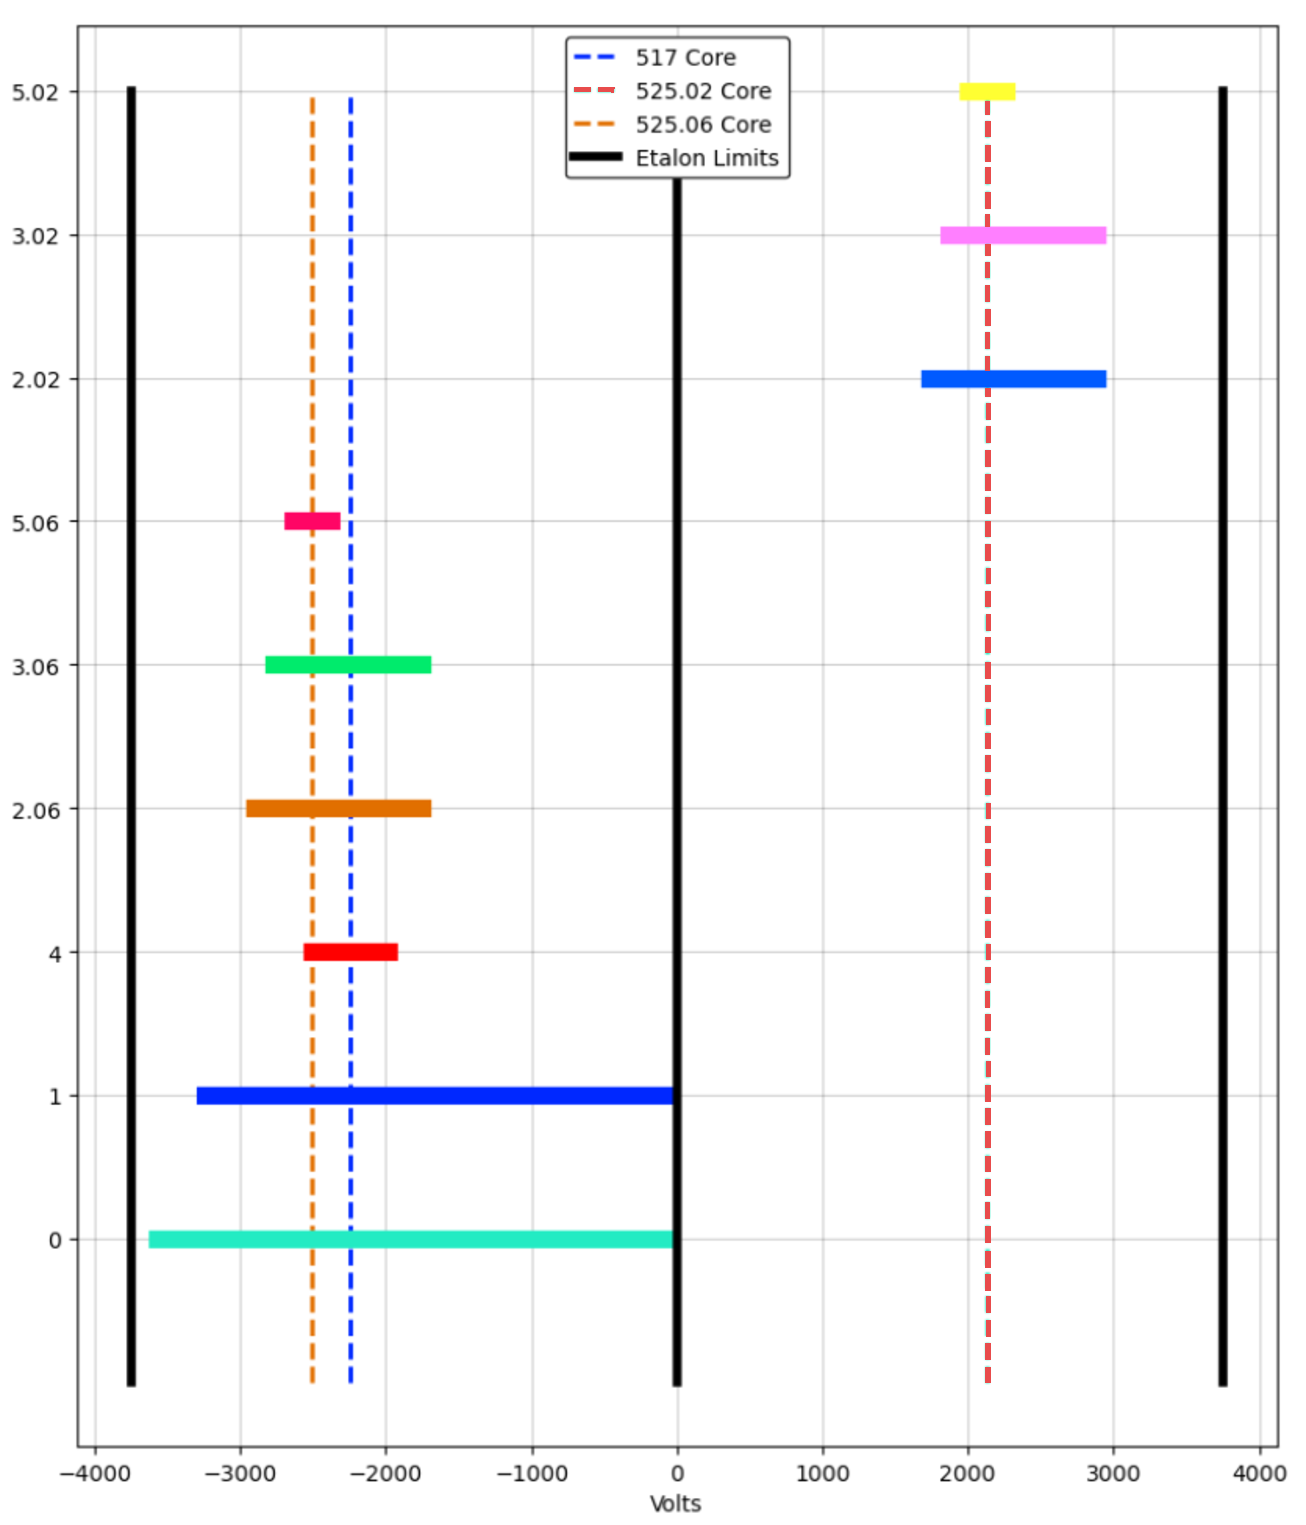
\includegraphics[width=\textwidth]{figures/Pipeline/obs_modes.pdf}
    \end{minipage}\hfill
    \begin{minipage}[c]{0.29\textwidth}
      \caption{
       Schematic representation of the voltage range covered by all observing modes. The dashed lines indicate the position of the line core as measured during the E2E tests performed at INTA in December 2021. The black lines represent the voltage limits that cannot be crossed in an observing mode.
       \label{fig_pipeline: Observing modes ranges}
      } 
    \end{minipage}
\end{figure}

Figure \ref{fig_pipeline: Observing modes ranges} presents a schematic representation of the voltage ranges for the observing modes when converting spectral sampling to volts. The black lines indicate the voltage boundaries that cannot be surpassed during an observation due to technical constraints. These limits are set at $\pm 3750$ V as the maximum and minimum values, with an additional limitation at 0 V, since a polarity change poses technical challenges that could not be addressed within an observation mode. These restrictions are significant in two cases: firstly, for Magnesium observation modes, specifically modes 1 and 0, where the continuum measurement is positioned as far from the core as possible, at -80 V, due to the 0 V crossing limitation. Secondly, these constraints are relevant when applying an etalon offset to shift the spectral positions of a particular observing mode, as the offset cannot cause the final positions to exceed these boundaries.

\subsection{Calibration modes}
An additional type of observing modes are also designed aimed at carrying out calibration observations. These calibration observing modes are more flexible than scientific ones, and allow for the configuration of several parameters to match the observations to the aim of the scientific observation. 

\begin{figure}[t]
    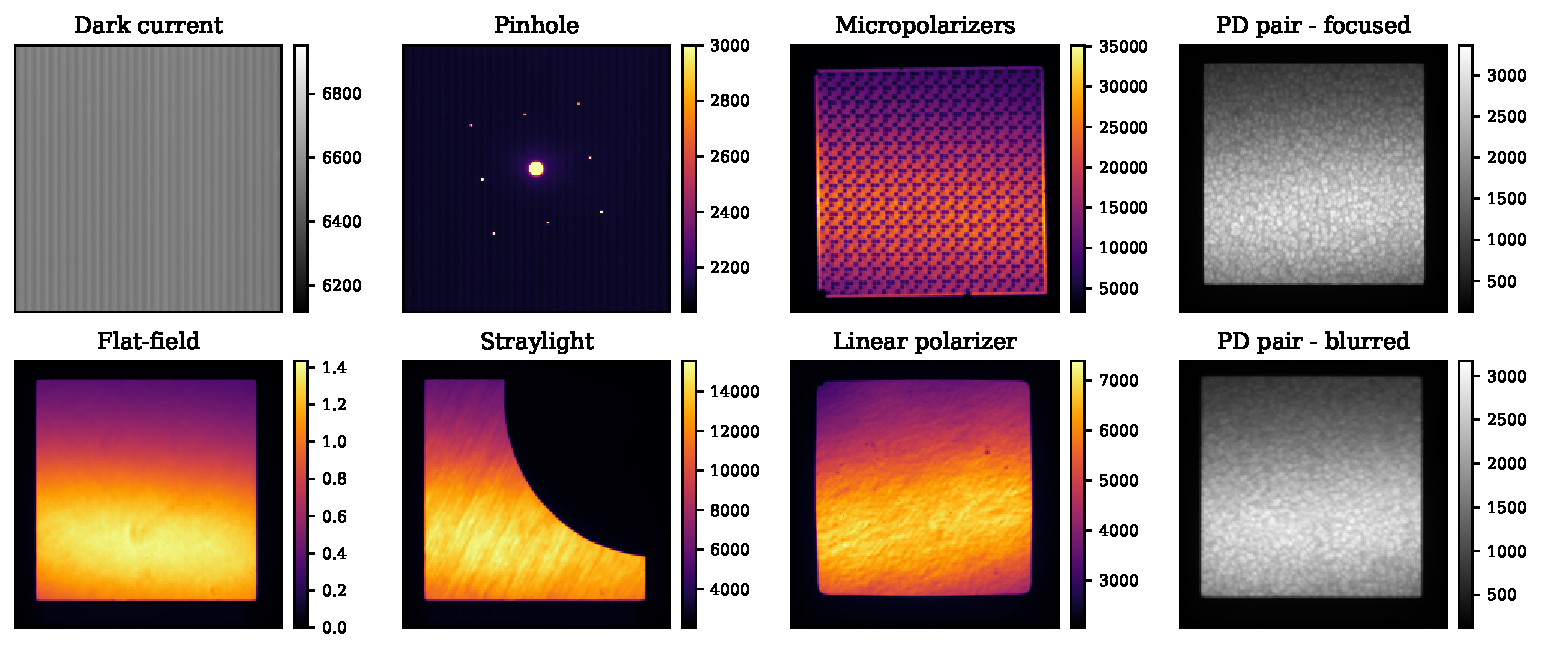
\includegraphics[width=\textwidth]{figures/Pipeline/cal_modes_examples.pdf}
    \caption{
      Examples of calibration observations. All images, with the exception of the flat-field, are presented in their raw format, without any manipulation or correction applied. The flat-field observation depicted corresponds to the first modulation of the continuum measurement obtained during a flat-field observation corresponding to observing mode 1. All data are belong to camera 1, and the colorbar is calibrated in digital counts save for the flat-field which is normalized to its mean value. }
      \label{fig_pipeline: cal_examples}
\end{figure}

\subsubsection{Flat-field observations}

One of the essential calibration procedures in any telescope-based astronomical observation is the acquisition of flat-field images. These observations are designed to measure intensity variations across the FoV, which arise from several factors, including intensity gradients induced by the etalon, dust particles, or pixel efficiency variations, among other sources. The aim is to capture a region with no discernible structure, ideally producing a uniformly flat intensity distribution. However, achieving such flat-field observations is not always straightforward, particularly for certain instruments. While ground-based telescopes can utilize twilight periods to observe areas of the sky devoid of stars, space-borne or balloon-borne solar telescopes, such as Sunrise III, are unable to the dame and must look for alternative methods. 

In Sunrise III, flat-field images are generated by deliberately blurring the solar image through rapid movements of the mirror. This process effectively removes any solar structure from the FoV when averaging out multiple blurred observations, resulting in a flat-field image devoid of solar features.

In the case of TuMag, flat-field observations are performed using a modified version of the nominal observing mode, where the $\lambda_{\text{rep}}$ is set to 4. Additionally, multiple consecutive instances ($N_{\text{reps}}$) of these observations are executed, typically 5 or 7. During data processing, a single flat-field is generated for each wavelength position and modulation state by averaging all corresponding observations.

Figure \ref{fig_pipeline: cal_examples} shows an example of a flat-field observation, for one camera, modulation and wavelength (bottom left panel). The image shows a clear deviation from flatness in the measurment, primarly due to the etalon intensity gradient, which accounts for the change in intensity between the brighter bottom half and the darker top half, and some minor inhomogeneities over the FoV. 

\subsubsection{Dark-current observations}

A second critical calibration procedure for any observation involving electronic cameras is the measurement of dark current. In the absence of incident photons, electrons within the camera's wells can still be randomly excited. This spontaneous excitation can be incorrectly interpreted as photon-induced counts when analyzing the data. Dark current observations are designed to characterize these random electronic excitations, which are primarily influenced by the camera's physical conditions, particularly temperature, so that they can be accurately subtracted from the final images.

For TuMag, dark current calibration involved capturing a series of 50 images with $N_a = 50$ with no light entering the instrument. As with flat-field observations, a single dark current frame for each camera is generated by averaging all individual observations. In the top left panel of fig. \ref{fig_pipeline: cal_examples} a dark current shot is depicted, characterized by the vertical strips pattern.  

\subsubsection{Linear polarizer and micropolarizers observations.}

TuMag's filter wheels are equipped with two targets designed to assess the instrument's polarimetric performance: a linear polarizer and a set of micropolarizers. Both targets are situated in the first filter wheel and are used in conjunction with the three distinct prefilters located in the second filter wheel. The linear polarizer serves to evaluate the polarimetric calibration, particularly by quantifying the level of cross-talk, as no circular polarization should be detected when using this target. The micropolarizers provide a more complete assessment, as they consist of multiple linear polarizers oriented at different angles. 

Observations with this targets are carried with the three prefilters, at a single wavelength, located in the continuum of each line. For each measurement, a vectorial modulation scheme is employed that allows for the derivation of the four stokes parameters. In the third column of figure \ref{fig_pipeline: cal_examples} observations of both targets are shown. 

\subsubsection{Pinhole Observations.}

Another calibration target included in the filter wheels is the pinhole target. This target blocks most of the light reaching the instrument, except for a few small holes arranged in a square-like pattern across the FoV, as shown in the top panel of the second column of figure \ref{fig_pipeline: cal_examples}. A larger hole is located at the center of the FoV, surrounded by eight smaller holes that trace a square with the central hole at its midpoint. These observations serve various purposes, including image alignment, detecting the presence of ghost images, or identifying etalon reflections, among other uses.

Pinhole observations are conducted similarly to those with polarizers, that is, in combination with the three prefilters at a single wavelength (the continuum of each line), but without applying any modulation.

\subsubsection{Straylight target.}

Not all the light that reaches the detector is necessarily the intended signal for a given observation. Some unwanted light, primarily originating from internal reflections along the optical path, may also reach the instrument. This unwanted contribution, known as straylight, contaminates the measurements by reducing contrast, lowering the S/N, and generally degrading the spectral, optical, and polarimetric performance of the instrument.

To address this contamination, TuMag performed a series of observations using a target that blocks part of the FoV (see the bottom panel of the second column of figure \ref{fig_pipeline: cal_examples}). By analyzing the dark region in these observations, it becomes possible to measure and model the straylight reaching the instrument, allowing for its subsequent removal from the data.

\subsubsection{Prefilter scans.}

TuMag observations are very sensible to spectral shifts either from the pre-filters or from the observed spectral line position. The shift of the pre-filters can happen due to changes in the physical conditions of the filter wheels such as changes in temperatures which spectraly shift the behavior of the pre-fitlers. The position of the pre-filter greatly affect the measurements as it reduces the intensity of the measurements that are obtained in the wings of the pre-filter. Due to solar rotation, or changes in the conditions of the etalon, although these are less likely, the spectral position at which the spectral lines are recorded can change. This effect is specially important in observing modes that require great spectral accuracy, such as the deep modes, where only three spectral positions close to the line core are employed. 

In order to verify the spectral behaviour of the prefilter, as well as the position of the spectral line, a series of observations were carried out, usually before and after the scientific observations, where a spectral scan with a rich spectral smapling was taken for all the pre-filters employed in the observation. These scans, measure the voltage range of the specific line with a sampling of 100V and without modulating. 

\begin{figure}[t]
    \begin{minipage}[c]{0.67\textwidth}
      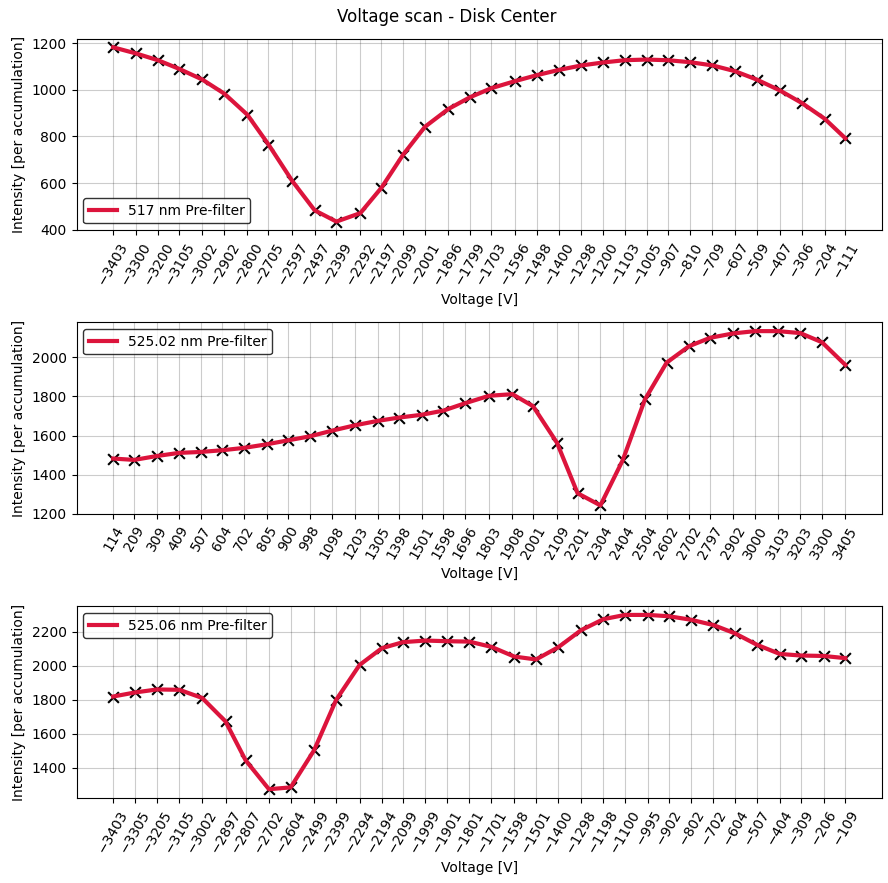
\includegraphics[width=\textwidth]{figures/Pipeline/Prefilter_scans.png}
    \end{minipage}\hfill
    \begin{minipage}[c]{0.29\textwidth}
      \caption{
       Schematic representation of the voltage range covered by all observing modes. The dashed lines indicate the position of the line core as measured during the E2E tests performed at INTA in December 2021. The black lines represent the voltage limits that cannot be crossed in an observing mode.
       \label{fig_pipeline:  prefilter_scans}
      } 
    \end{minipage}
  \end{figure}


\subsubsection{Phase diversity.}

Lastly, TuMag is equipped with the capability to perform phase diversity for image reconstruction. As discussed in previous chapters, applying image reconstruction techniques is essential to meet the optical quality requirements. To this end, TuMag includes a PD plate in the first filter wheel that introduces a known defocus in the images. Capturing images with and without this plate enables the computation of the instrument's PSF, which can then be deconvolved from the data.

PD measurements require quasi-simultaneous pairs of aberrated and unaberrated images. Therefore, TuMag's PD observations consist of a series of 32 or 40 rapid, non-accumulated shots with the PD plate, followed by a corresponding series without the PD plate. The feasibility of this sequential scheme for phase diversity techniques has been confirmed in \cite{PD_sequential}. A pair of focused-defocused images of quiet-sun observations is shown in the last column of figure \ref{fig_pipeline: cal_examples}.

\section{Timelines}

The operations of Sunrise III were designed to be nearly autonomous to ensure synchronization between the scientific instruments, the telescope, and the CWS. Given the limited time available for the observation campaign, this autonomy also helps to speed up operations, thus enabling more observation programs to be accommodated within the mission's duration.

The Sun is a highly dynamic system, exhibiting a wide range of behaviors and phenomena, from large-scale structures such as active regions, sunspots, and flares, to smaller, quiet Sun structures where interactions at small scales drive the evolution of magnetic flux. This diversity, observable in various spectral lines and across different regions of the solar disk, demands multiple observations with distinct characteristics.

Prior to the first flight of Sunrise III in 2022, a series of timelines were developed to program both calibration and scientific observation blocks. These timelines were carefully designed by the Sunrise Science Team, taking into account the 70 observing proposals submitted for Sunrise, in order to prioritize observations that met the requirements of the majority of these proposals.

Observing proposals that could be fulfilled by targeting the same solar feature, while considering its disk position, were grouped into a single timeline. Each timeline included not only the necessary scientific observation blocks but also the required calibration observations to ensure data accuracy. Thus, timelines consist of a sequence of scientific and calibration observation blocks. The observing blocks within a timeline could vary in content depending on the scientific objectives and the status of the other instruments involved.

For simplicity, operations related to SCIP and SUSI will be excluded from the discussion, save for a few important remarks. In the case of TuMag, each observing block was composed either of a combination of two observing modes executed consecutively, or a single observing mode repeated throughout the block.  

\begin{figure}
  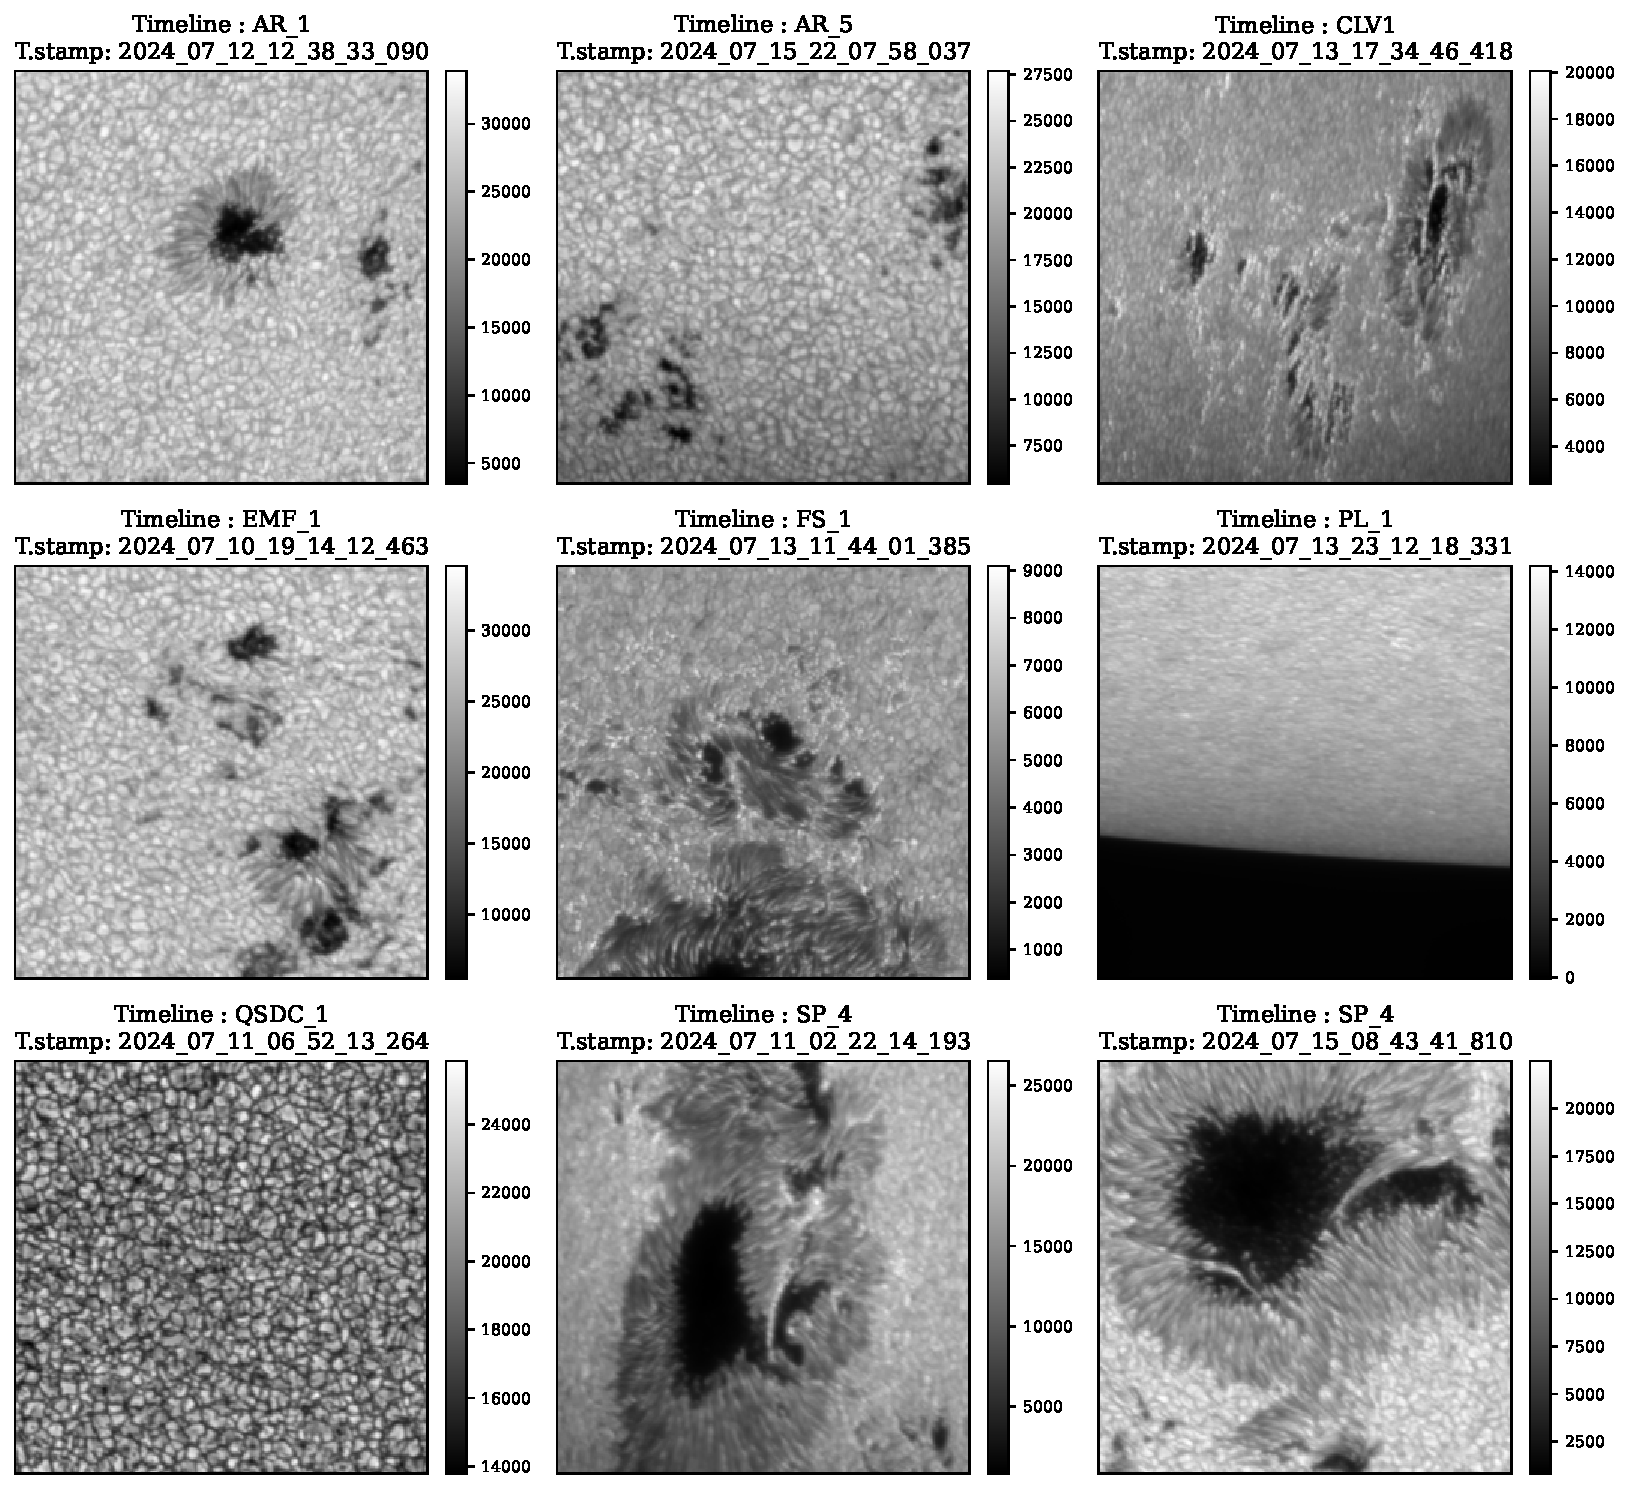
\includegraphics[width=\textwidth]{figures/Pipeline/timelines_Examples.pdf}
  \caption{
    Continuum images of the first modulation of the first observation mode from different timelines. The image shown has been flat-fielded and dark-corrected. The timestamp provided corresponds to the first image of the observation mode. The colorbar is given in counts.}
    \label{fig_pipeline: timeline_examples}
\end{figure}

The timelines of the Sunrise III observation campaign can be gropued in the following blocks: 

\begin{itemize}
  \Myitem Quiet Sun observations at disk center (QSDC), as the name implies , focus in regions near the solar disk center that are free from significant solar activity. These timelines typically involvve long series of observations aimed at studying the small-scale structure and magnetic flux evolution in the quiet Sun. 
  
  There are four distinct timelines in this category: three standard timelines, which ewmploy the nominal observing modes, and a different timeline, the (QSDC{\_}HC). This timeline employs high-cadence variations of the standard observing modes specifically designed to enhance the temporal resolution between images, which is crucial for helioseismology techniques.
  \Myitem Sunspot observations (SP) are specifically designed to study sunspots. There are four different timelines for this purpose. Some of these are short programs used to track the same sunspot over multiple days, with the goal of studying the evolution and decay of the sunspot. Others are more extensive programs aimed at examining, in greater detail, the magnetic activity of sunspots and their penumbral structures.
  \Myitem Polar observations (PL) target the region close to the limb in both poles of the Sun. These areas are of special interest due to their distinct magnetic behavior compared to the disk center. Additionally, these regions provide the opportunity to measure faint signals outside the main solar disk, such as spicules in the lower chromosphere, observed outside the continuum disk of iron. Two different instances of these timelines are conceived in the observation campaign, mostly differenciated in TuMag by the selected spectral lines.
  \Myitem East and West limb (EW) observations are designed to target the equatorial regions of the solar limb. In addition to exhibiting magnetic structures distinctly different from those observed at the poles, the reason for having a separate timeline from the PL timelines lies in the orientation and technical constraints related to SCIP and SUSI's slits. The relative positioning of the regions and the inclination of the telescope introduce unique challenges. In these EW observations, the spectrometer slits are aligned parallel to the limb, contrasting with the PL timelines, where the slit is positioned perpendicular to the limb.
  \Myitem Active regions (AR) observations are designed to study areas exhibiting solar activity, excluding those specifically focused on in the sunspot programs. These observations typically consist of two-hour series, employing the standard combination of the iron 525.02 nm and magnesium lines, using modes 1 and 2.02, which represent the most common observation block for TuMag. Although five different AR timelines were planned for the Sunrise campaign, only three were executed.
  \Myitem Emergence flux (EMF) programs are specifically desinged to study active regions that exhibit a large flux emercence. For TuMag, the observation blocks are shared with those of a the AR programs, namely, the combination of mode 1 and 2.02 for series of around 2 hours. 
  \Myitem Full spectral scan (FS) observations are primarily designed for SUSI and SCIP, where their complete set of spectral bands is utilized. These scans are intended to be carried out in both quiet Sun and active regions. For TuMag, FS observations consist of long series focusing on the iron spectral line in quiet Sun regions, while in active regions, they include a combination of iron and magnesium observations.
  \Myitem The flares programs (FL) were designed for target oportunities of a flaring region. These programs were intended to be activated only when an active region showed signs of flaring. For TuMag, the observations during these programs consist of the standard combination of iron 525.02 nm and magnesium spectral lines.
  \Myitem Center-to-limb variation (CLV) observations were intended to target regions of the solar disk characterized by $\mu$ values that had not been previously observed. The parameter $\mu$, defined as the cosine of the angle between the surface normal and the observer's line of sight, serves as a useful indicator of a region's proximity to the disk center. Specifically, $\mu$ ranges from 1 at the disk center to 0 at the limb \citep{thompson2006coordinate}. Conducting CLV observations at previously unmeasured $\mu$ values enables us to capture data from different regions across the disk, facilitating studies of how observational features vary with their position on the disk. 
\end{itemize}

During the Sunrise III observation campaign, 38 timelines were run, including calibration timelines in addition to the scientific programs presented here. Some examples of the different targets employed during the campaign are shown in fig. \ref{fig_pipeline: timeline_examples}.  A detailed record of TuMag's observations can be found online both in the pipeline's repository and in TuMag's official data website\footnote{\url{https://www.uv.es/jublanro/tumag_data_test.html}}.  

\section{Pipeline}

When light traverses any astronomical instrument, the optical components it encounters between the aperture and the detector can alter the light in unintended ways. These modifications give rise to artifacts that must be corrected prior to the scientific exploitation of the observations, as they can falsify the results if left unaddressed. The process of eliminating these spurious effects is typically referred to as data reduction and is specific to each instrument, as different optical elements require different corrections.

As a spectropolarimeter, TuMag's final data product are not \textit{simply} the measured images but the Stokes components of the incoming light, when either modulation scheme is employed. Consequently, TuMag's data pipeline must not only remove all instrumental artifacts but also include the necessary procedures to demodulate the data and derive the Stokes components for each wavelength along the spectral line.

This section presents the software specifically developed for this purpose. The discussion will cover the various steps that data must undergo before becoming science-ready, as well as the tools created to facilitate this process. All codes related to TuMag's pipleine are publicly available in a GitHub repository\footnote{\url{https://github.com/PabloSGN/TuMags_Reduction_Pipeline}}, and it is important to note that this software is still under development at the time of writing this thesis.

\subsection{Standard data reduccion process.}

We have divided the discussion of the pipeline in two sections, the so-called "standard data reduction process" and the extra calibration blocks. The first being all the steps that are mandatory to process am individual observing mode and produce the Stokes components with the most basic corrections. These are the minimal steps to produce data that can start to be analyzed scientifically. The second block is comprised of all the additional corrections and considerations that may or may not be applied to the data, depedning on the nature of the observation. While this division may not be entirely accurate, as science-ready data will likely require the application of additional calibrations, such as image reconstruction, for instance, we have adopted it to simplify the discussion of the pipeline.

All data corresponding to an observing mode whose final product consists of the Stokes components of the incoming light (i.e., all nominal modes except for the 0s mode) must follow the standard reduction process. This process is illustrated in the block diagram in fig. \ref{fig_pipeline: block_diagram} and consists of the following steps:
\begin{enumerate}
  \item Dark current processing. 
  \item Flat-fielding processing.
  \item Camera's alignment computation. 
  \item Processing of observing mode images (dark-current corrected). 
  \item Apply flat-field correction.
  \item Demodulation. 
  \item Cross-talk correction and cameras combination.
  \end{enumerate}

\begin{figure}[t]
  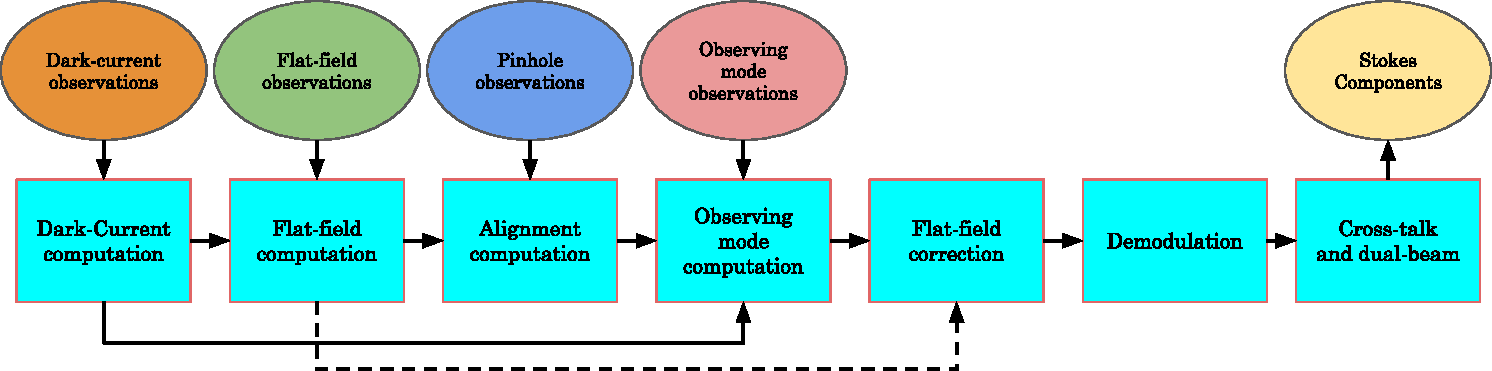
\includegraphics[width=\textwidth]{figures/Pipeline/block_diagram.pdf}
  \caption{
    Block diagram of the standard reduction process: Blue boxes represent the individual steps that make up the reduction, while ellipses indicate the different sets of observations and the final product (yellow ellipse). }
    \label{fig_pipeline: block_diagram}
\end{figure}

The data reduction process begins with the dark-current processing, which involves averaging all individual dark frames within a specific set to generate a single dark-current frame per camera. This dark current is then subtracted from all images used in the reduction, including flat-fields, pinholes, and scientific observations, after rescaling the dark-current to the appropriate number of accumulations.

The second step is the flat-field computation. These observations, as previously mentioned, are a modified version of the nominal mode with an increased $\lambda_{\text{rep}}$ and are repeated $N_{\text{rep}}$ times. The processing involves averaging all images taken at a specific wavelength for the same modulation. Thus, $\lambda_{\text{rep}} \times N_{\text{rep}}$ images are averaged to produce a single flat-field frame. To maintain spectral line information, flat-fields are normalized to their mean value, as flat-fields taken at the line core have lower intensity than those in the continuum. The goal is to correct intensity variations within a single frame without altering relative intensities across different spectral points.

Since TuMag operates in a dual-beam configuration, data from both cameras must be combined during processing. However, the images from each camera are not initially aligned. To determine the camera alignment, a two-dimensional cross-correlation is performed using the pinhole target from both cameras. Additionally, the field stop position is required for alignment, as TuMag's detectors are larger than its FoV. A specific function identifies the field stop positions from the processed flat-fields, marking the boundary between dark pixels and those within TuMag's FoV. Figure XX provides a representation of both the pinhole alignment and the field-stop finder.

\begin{figure}[t]
  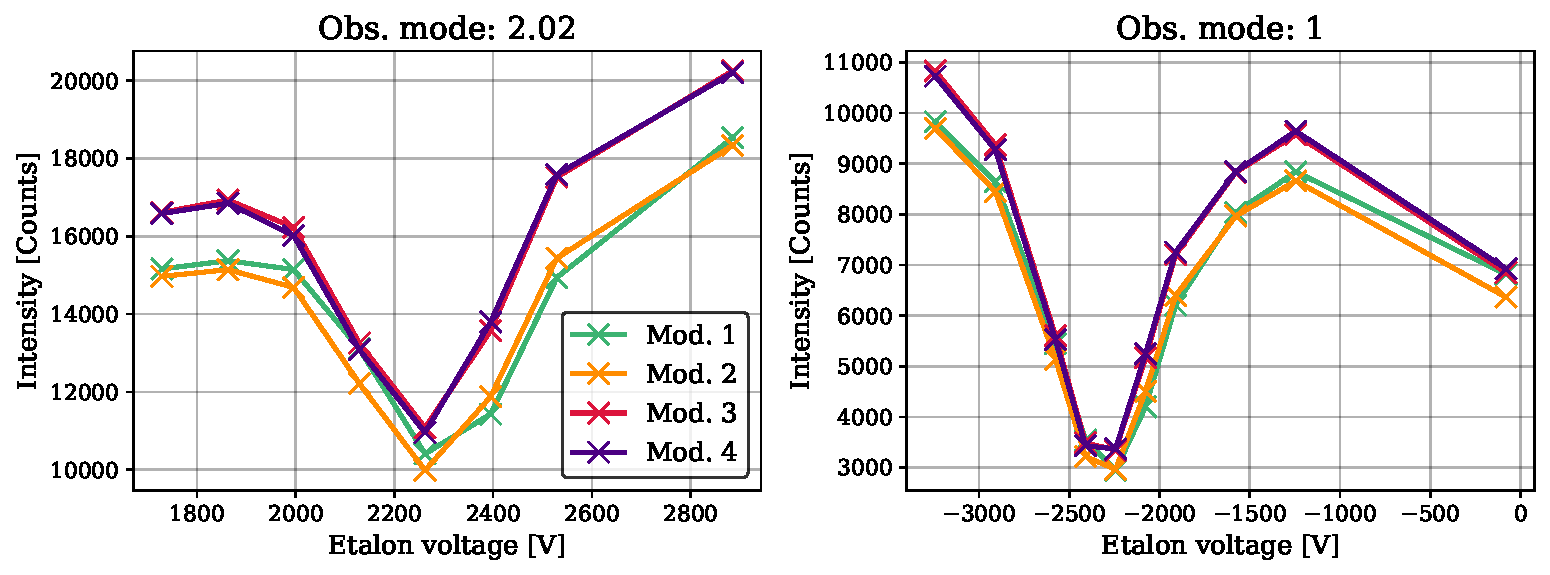
\includegraphics[width=\textwidth]{figures/Pipeline/Spectral_scans_ecample.pdf}
  \caption{
    Block diagram of the standard reduction process: Blue boxes represent the individual steps that make up the reduction, while ellipses indicate the different sets of observations and the final product (yellow ellipse). }
    \label{fig_pipeline: spectral_scans}
\end{figure}


Having computed the dark-current and the flat-fields, the scientific observations can be corrected by substracting the dark-current and dividing the resulting image by the flat-field of the corresponding wavelength and modulation. 

With the dark-corrected and flat-fielded observations, the stokes components can be computed. The demodulation is carried at each wavelength separately and consists on the matrix multplication of the demodulation matrix and the four stokes components:
\begin{equation}
  \begin{pmatrix}
  I \\
  Q \\
  U \\
  V
  \end{pmatrix} = 
  \underbrace{\begin{pmatrix} 
      d _ {00} & d _ {01} & d _ {02} & d _ {03} \\ 
      d _ {10} & d _ {11} & d _ {12} & d _ {13} \\
      d _ {20} & d _ {21} & d _ {22} & d _ {23} \\
      d _ {30} & d _ {31} & d _ {32} & d _ {33} 
  \end{pmatrix}}_ {\textbf{D}}
  \begin{pmatrix}
    I _ {1} \\
    I _ {2} \\
    I _ {3} \\
    I _ {4}
    \end{pmatrix} \ \ , 
    \label{pipeline: Demod}
\end{equation}
\textcolor{red}{Modo Longitudinal??}
where the matrix D is the inverse of the modulation matrix of the corresponding camera and pre-filter that were computed during the calibrations (see sec. \ref{sect:tumag_cal polarimetric}).

From the matrix multiplication the stokes components for each camera are derived. However, the demodulation is never perfect, due to small deviations of the demodulation matrix from the real one, or instrumental artifacts that have been uncorrected by the flat-fielding. These defects result in a contaminated stokes components, where information from one component appears in other components, typically from Stokes I into Q, U, and or V. Nonetheless, these contamination, known as cross-talk, can be extracted from the data. 

The cross-talk correction is a manual process since different data sets require different corrections. For instance, some data sets may not show contamination from I to U while others do. Moreover, the correction might require to be applied using the information from the whole FoV or only of a small region. Thus, this is a correction that has to be carefully applied and its hard to standarize to the whole set of observations. However, the concept of the correction is the same. 

The correction of the cross-talk from I to any other component starts by measuring the relation between the two components by fitting through a least-squares method, a polynomial of first order in order to compute the tendency, if there is one. Once this relation has been stablished, and the strength of the cross-talk (\textit{i.e.} the value of the slope) measured, the correction is applied by simply, removing the tendency of the data: 

\begin{equation}
  S_{corr} = S_{orig} - (I_{orig} * a + b),
\end{equation}
where the relation between the stokes component $S_{orig}$ and stokes I $I_{orig}$ has been fitted to the line: $S_{orig} =  I_{orig} * a + b$

\subsection{Extra calibration blocks.}

\subsection{Image reconstruction.}
\subsubsection{Linear polarizer calibration.}
\subsubsection{Micropolarizerss calibration.}
\subsubsection{Prefilter scans.}

